\documentclass[preview,border=5pt]{standalone}
\usepackage{teaching}
\begin{document}

\centering

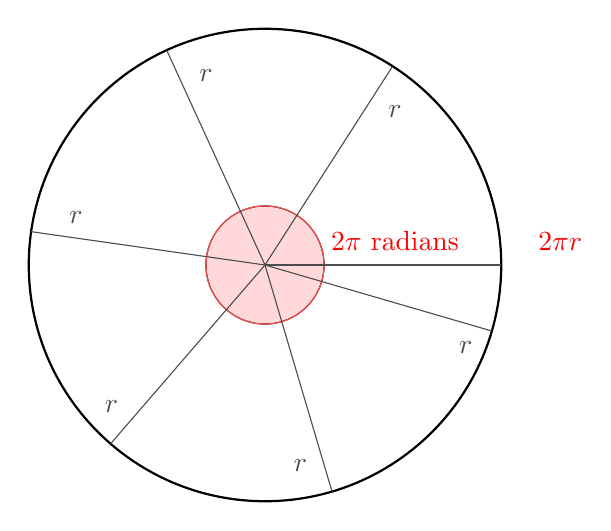
\begin{tikzpicture}[yscale=1,xscale=1,scale=1.5,inner sep=0.1mm, label distance=1.5mm]

%\draw[black!30!white, ->] (-3,0) -- (3,0);
%\draw[black!30!white, ->] (0,-3) -- (0,3);
%\node(t) at (3.15,0) [color=black!50!white] {$x$};
%\node(t) at (0,3.15) [color=black!50!white] {$y$};
\draw[thick] (0,0) circle (2);
\draw[fill=red!15!white] (0,0) circle (0.5);
\draw[color=red!70!white] (0,0) circle (0.5);
\draw[black!70!white] (0,0) -- (2,0);
\draw[black!70!white] (0,0) -- (1.08060461174,1.68294196962);
\draw[black!70!white] (0,0) -- (-0.83229367309,1.81859485365);
\draw[black!70!white] (0,0) -- (-1.9799849932,0.28224001612);
\draw[black!70!white] (0,0) -- (-1.30728724173,-1.51360499062);
\draw[black!70!white] (0,0) -- (0.56732437092,-1.91784854933);
\draw[black!70!white] (0,0) -- (1.9203405733,-0.55883099639);
%\draw[red, ->] (2.2,0) arc (0:57.2958:2.2cm);
%\node(r) at (1,-0.2) [color=red] {$r$};
\node(j) at (1.1,1.3) [color=black!70!white] {$r$};
\node(j) at (-0.5,1.6) [color=black!70!white] {$r$};
\node(j) at (-1.6,0.4) [color=black!70!white] {$r$};
\node(j) at (-1.3,-1.2) [color=black!70!white] {$r$};
\node(j) at (0.3,-1.7) [color=black!70!white] {$r$};
\node(j) at (1.7,-0.7) [color=black!70!white] {$r$};
\node(j) at (1.1,0.2) [color=red] {$2\pi$ radians};
\node(j) at (2.5,0.2) [color=red] {$2\pi r$};
\bonusspiral[red, ->](0,0)(0:0)(2.2:2.4)[1];

\end{tikzpicture}

\end{document}